Pour savoir si les réseaux $\mathcal{S}$MorphNetTanh sont des réseaux d'intérêt, au-delà de l'amélioration de la formulation asymptotique des couches $\mathcal{S}$MorphTanh quand $\alpha \rightarrow -\infty$ par rapport à celle des couches $\mathcal{S}$Morph telle que vue précédemment, il faut étudier les performances de ces nouveaux réseaux sur un ensemble d'expériences et comparer leurs résultats à ceux des réseaux $\mathcal{S}$MorphNet simples. \\

\vspace{-1.6mm}
%Pour comparer avec rigueur la précision et l'efficacité des deux réseaux $\mathcal{S}$MorphNet et $\mathcal{S}$MorphNetTanh, ...
\noindent Dans cet objectif, on reprend le même protocole d'expérimentation que dans l'état de l'art, où l'on étudie l'état des réseaux après leur entraînement avec certaines métriques. En particulier : 

\vspace{0.4mm}
\begin{itemize}%[leftmargin=*]
    \item[$\bullet$] on reprend les quatre mêmes métriques d'évaluation de la performance des réseaux que dans l'état de l'art (partie 2.4) ;
    \item[$\bullet$] on reste sur la banque d'images en niveaux de gris MNIST ;
    \item[$\bullet$] on fait cette fois-ci six runs par expérience, au lieu de cinq ;
    \item[$\bullet$] on considère cette fois huit fonctions structurantes, en prenant les six précédentes de l'état de l'art, et en y ajoutant une fonction structurante diagonale asymétrique \textit{adiag} et une autre plate aléatoire \textit{brand}.
\end{itemize}

\vspace{2.2mm}
On résume, comme dans l'état de l'art, les résultats de l'ensemble des expériences en quatre groupes : le premier pour les expériences avec l'érosion pour opération cible (réseaux à une couche morphologique), le deuxième avec la dilatation (1 couche), le troisième avec l'ouverture (2 couches), et le dernier avec la fermeture (2 couches). \\

%\vspace{-0.6mm}
Pour l'érosion sur des réseaux à une couche, on obtient les résultats suivants :

% figure
\vspace{4.0mm}
\begin{figure}[ht]
  \begin{center}
    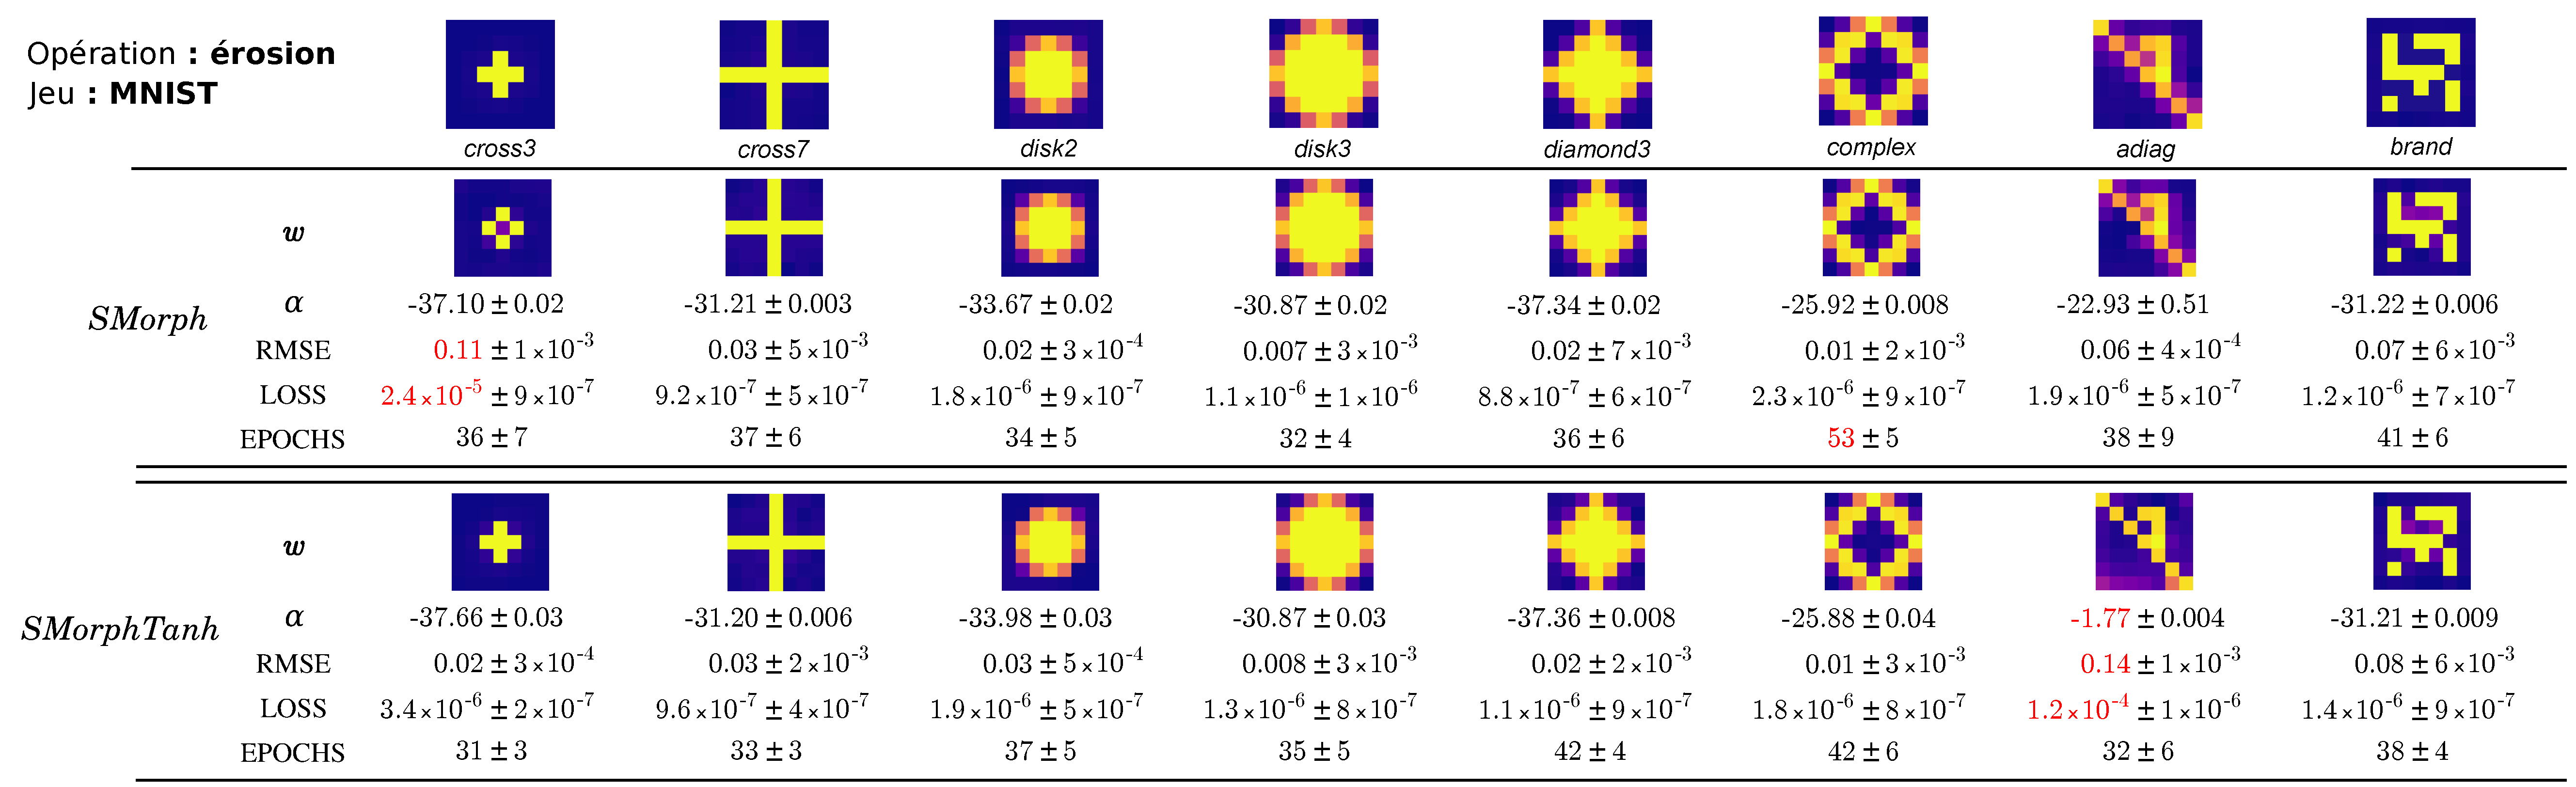
\includegraphics[width=1.00\textwidth]{parts/3-contributions/A-reseaux_smorphTANH/figures/t_erosion_mnist.pdf}
    \vspace{-2.0mm}
    \caption{ \centering Comparaison des poids appris et des moyennes et écarts-types des métriques $\alpha$, \textit{RMSE}, \textit{loss} et nombre d'époques, et ce sur six runs, entre $\mathcal{S}$Morph et $\mathcal{S}$MorphTanh à une couche, pour les huit fonctions structurantes cibles et l'opération d'\textbf{érosion}.}
    \label{fig:SMvsSMTH_erosion_mnist}
  \end{center}
\end{figure}


\newpage

\noindent En rouge sont notées les moins bonnes performances moyennes du réseau par rapport à l'autre (grandes moyennes). En vert, les résultats instables (grands écarts-types). \\

\vspace{2mm}
%Pour l'opération cible de dilatation sur des réseaux à une seule couche morphologique, on obtient les résultats suivants : \\
Pour la dilatation sur des réseaux à une couche, on obtient les résultats suivants : \\

% figure
\vspace{2.5mm}
\begin{figure}[ht]
  \begin{center}
    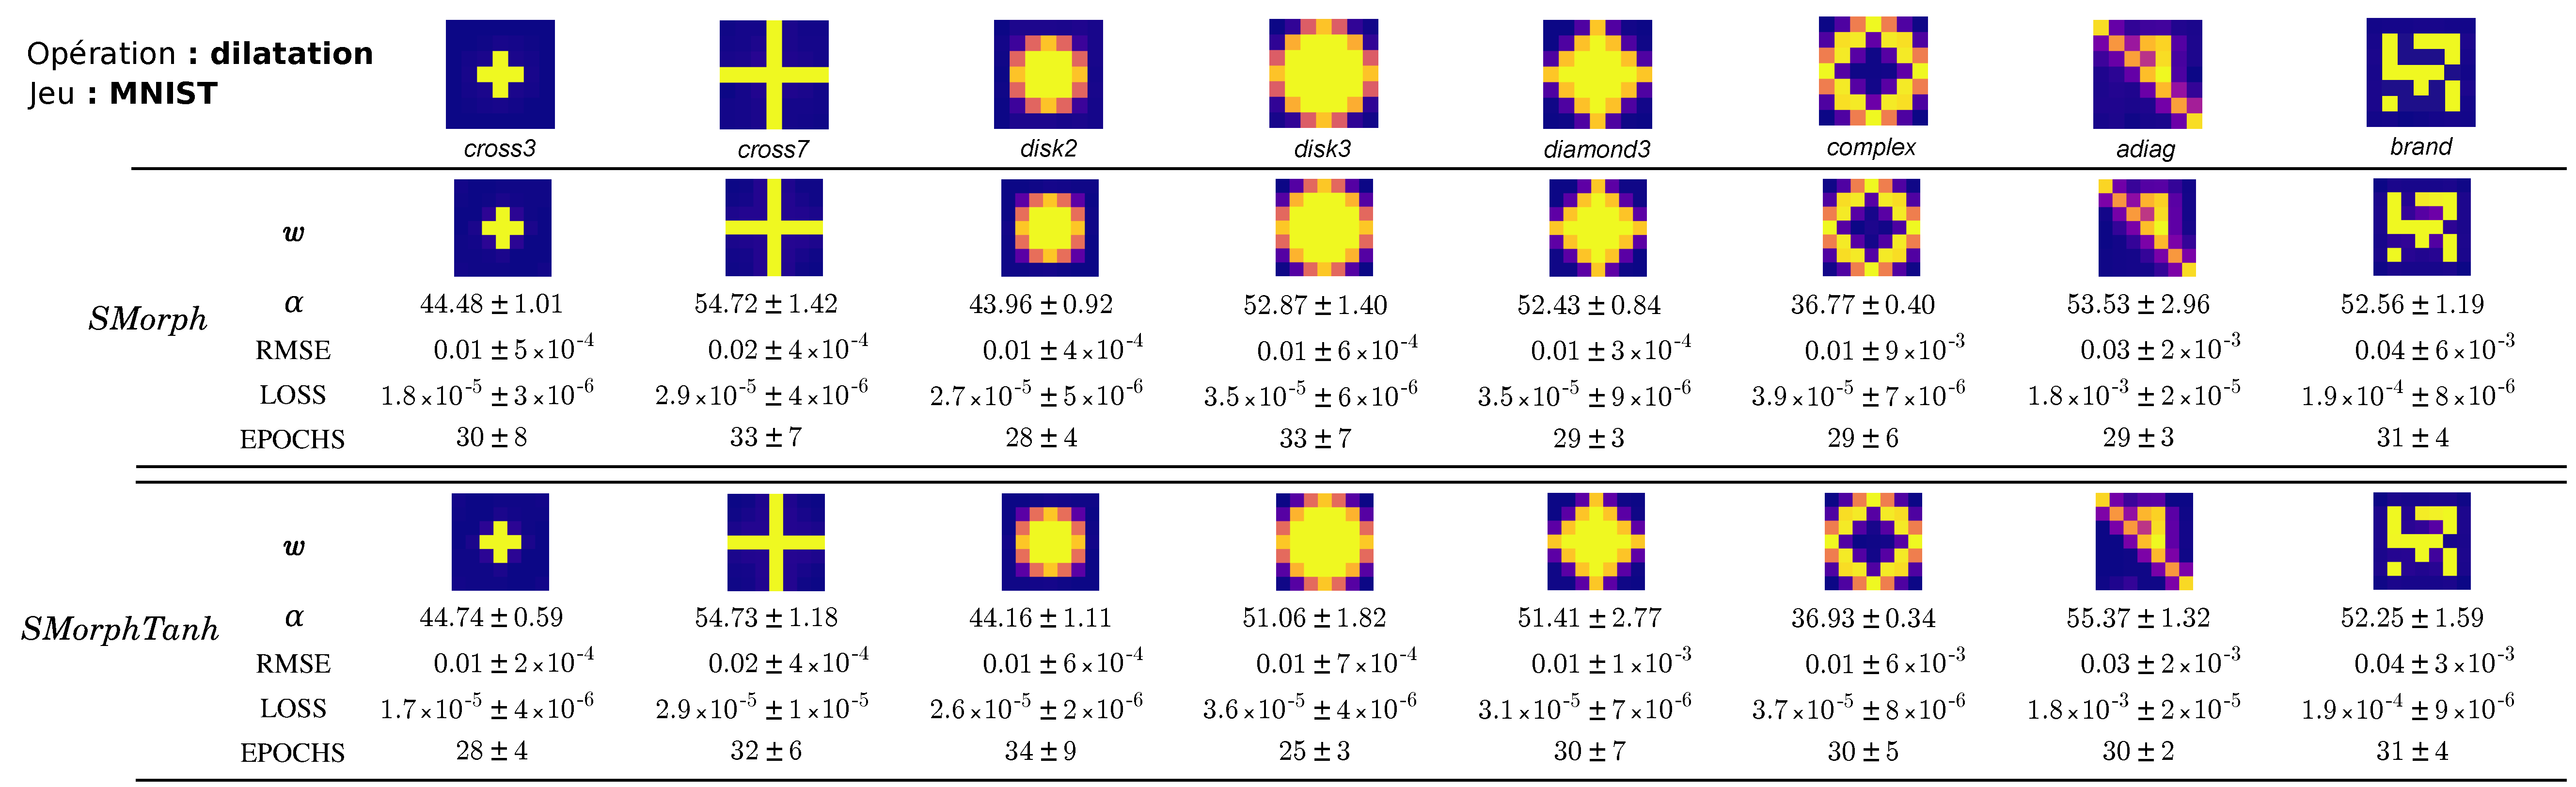
\includegraphics[width=1.00\textwidth]{parts/3-contributions/A-reseaux_smorphTANH/figures/t_dilation_mnist.pdf}
    \vspace{-2.0mm}
    \caption{ \centering Comparaison des poids appris et des moyennes et écarts-types des métriques $\alpha$, \textit{RMSE}, \textit{loss} et nombre d'époques, et ce sur six runs, entre $\mathcal{S}$Morph et $\mathcal{S}$MorphTanh à une couche, pour les huit fonctions structurantes cibles et l'opération de \textbf{dilatation}.}
    \label{fig:SMvsSMTH_dilation_mnist}
  \end{center}
\end{figure}

\vspace{1.5mm}
%Pour l'opération cible d'ouverture sur des réseaux à deux couches morphologiques, on obtient les résultats suivants : \\
Pour l'ouverture sur réseaux à deux couches, on obtient les résultats suivants : \\

% figure
\vspace{2.0mm}
\begin{figure}[ht]
  \begin{center}
    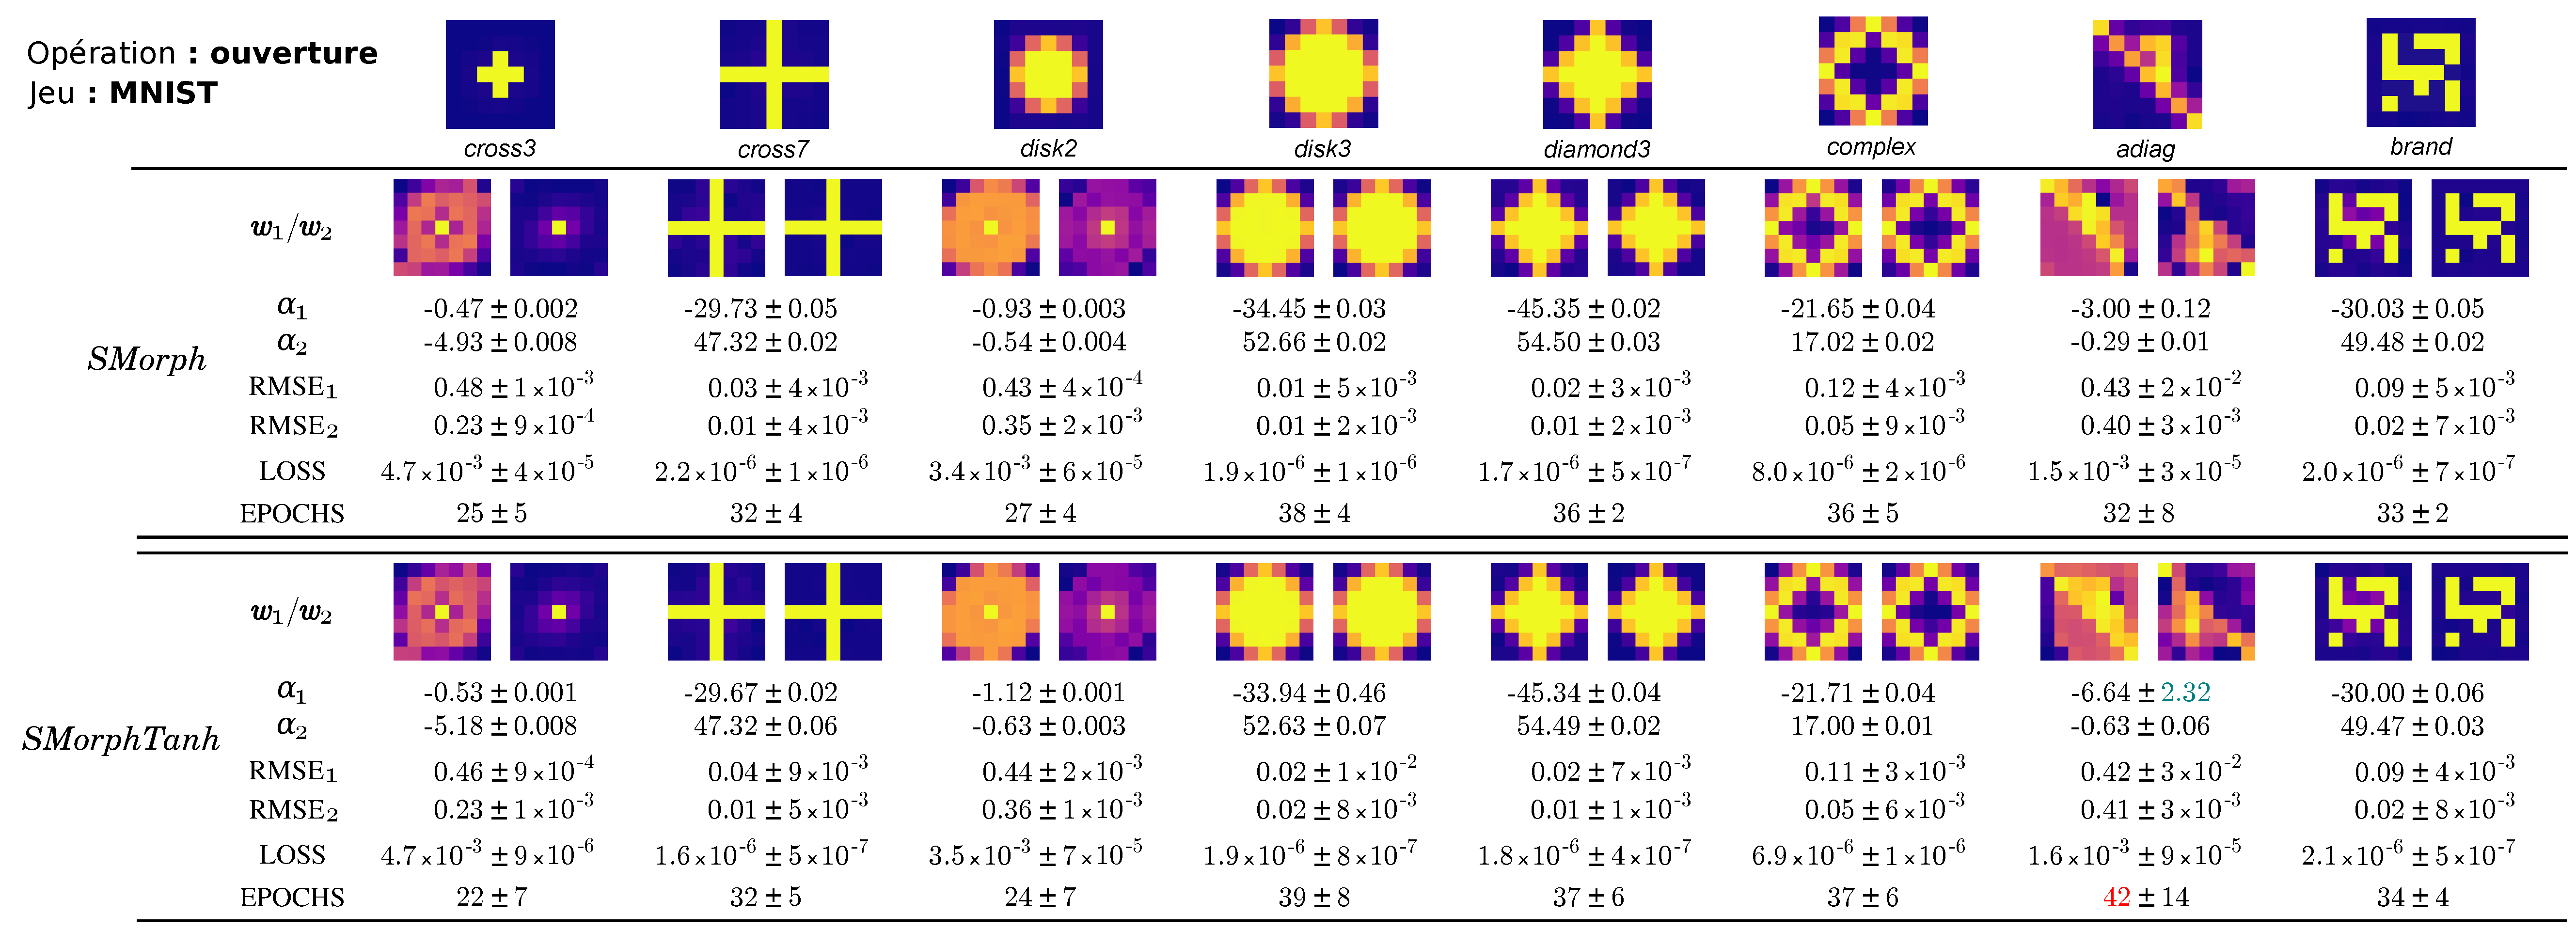
\includegraphics[width=1.00\textwidth]{parts/3-contributions/A-reseaux_smorphTANH/figures/t_opening_mnist.pdf}
    \vspace{-2.0mm}
    \caption{ \centering Comparaison des poids appris et des moyennes et écarts-types des métriques $\alpha$, \textit{RMSE}, \textit{loss} et nombre d'époques, et ce sur six runs, entre $\mathcal{S}$Morph et $\mathcal{S}$MorphTanh à deux couches, pour les huit fonctions structurantes cibles et l'opération d'\textbf{ouverture}.}
    \label{fig:SMvsSMTH_opening_mnist}
  \end{center}
\end{figure}


\newpage

%Pour l'opération cible de fermeture sur des réseaux à deux couches morphologiques, on obtient les résultats suivants : \\
Pour la fermeture sur réseaux à deux couches, on obtient les résultats suivants : \\

% figure
\vspace{2.0mm}
\begin{figure}[ht]
  \begin{center}
    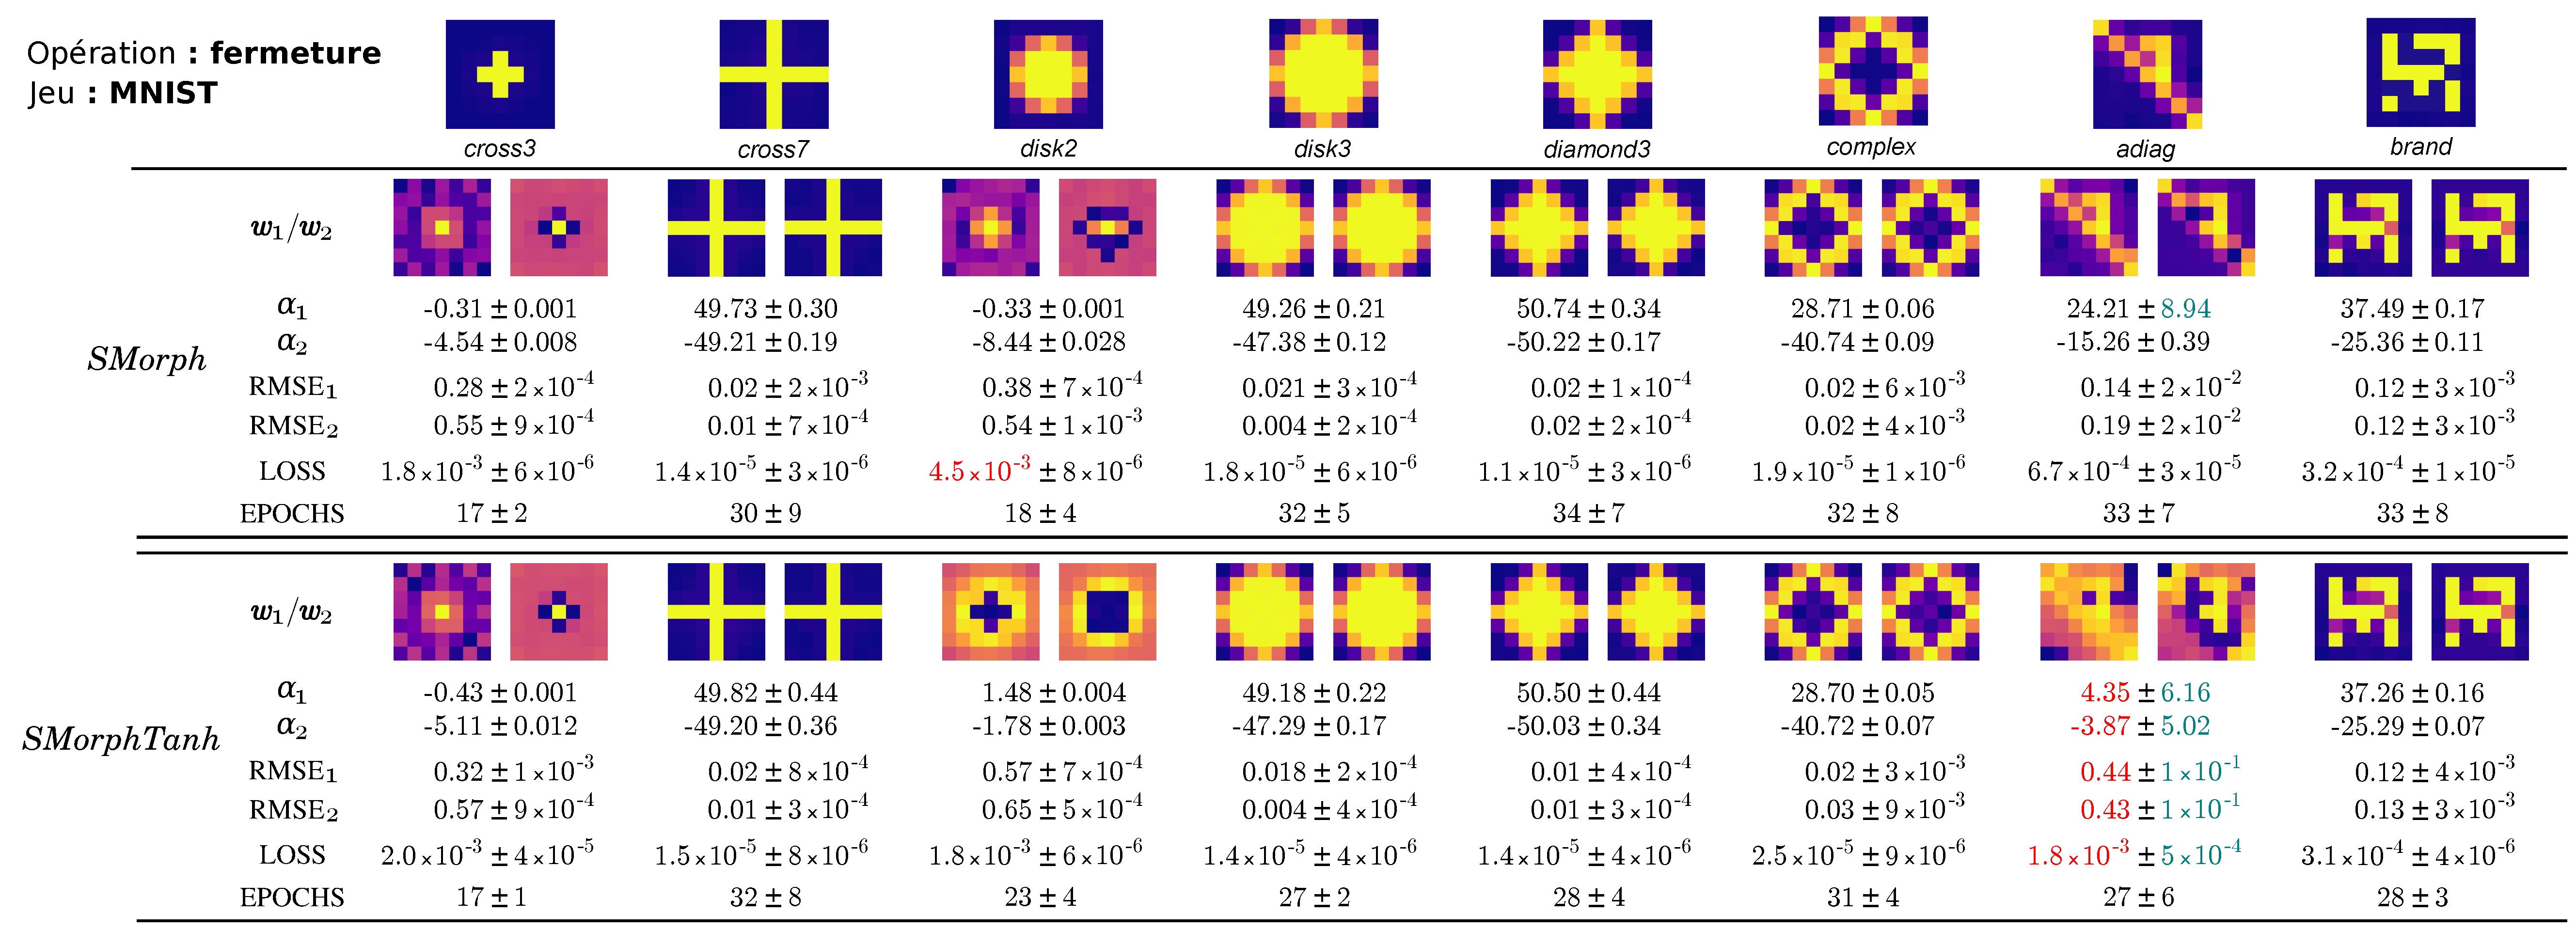
\includegraphics[width=1.00\textwidth]{parts/3-contributions/A-reseaux_smorphTANH/figures/t_closing_mnist.pdf}
    \vspace{-2.0mm}
    \caption{ \centering Comparaison des poids appris et des moyennes et écarts-types des métriques $\alpha$, \textit{RMSE}, \textit{loss} et nombre d'époques, et ce sur six runs, entre $\mathcal{S}$Morph et $\mathcal{S}$MorphTanh à deux couches, pour les huit fonctions structurantes cibles et l'opération de \textbf{fermeture}.}
    \label{fig:SMvsSMTH_closing_mnist}
  \end{center}
\end{figure}


\vspace{-3.2mm}

\vspace{-1.6mm}
Pour les réseaux à une couche : 
il n'existe pas de grandes différences entre les résultats portés par $\mathcal{S}$MorphNet et ceux portés par $\mathcal{S}$MorphNetTanh. L'ensemble des résultats semble plutôt bon pour ces deux réseaux uni-couche, aussi bien au niveau de la \textit{loss}, de la \textit{RMSE}, du signe et de l'amplitude de $\alpha$, et de la vitesse de convergence. Il existe toutefois deux expériences dont les résultats entre ces deux réseaux divergent légèrement : la première avec \textit{cross3} où $\mathcal{S}$MorphNetTanh semble meilleur en terme de \textit{RMSE} et de \textit{loss} ; la seconde avec \textit{adiag} où cette fois $\mathcal{S}$MorphNet semble meilleur. \\

\vspace{-1.8mm}
\noindent Pour les réseaux à deux couches : 
on retrouve les mêmes problèmes de convergence avec \textit{cross3} et \textit{disk2} que dans l'état de l'art (partie 2.4). On remarque que \textit{adiag} pose ici également des problèmes pour les deux réseaux. Cependant, là où $\mathcal{S}$MorphNet et $\mathcal{S}$MorphNetTanh se comportent de la même manière sur ces trois structures cibles avec l'ouverture, ils se comportent plutôt différemment avec la fermeture. Pour les autres structures, les deux réseaux donnent des résultats à la fois bons et similaires. \\

\vspace{-1.8mm}
\noindent Ces expériences ont été réalisées avec une autre banque d'images, FashionMNIST, et les mêmes conclusions de similarité d'efficacité des deux réseaux ont pu être établies. \\
%malgré quelques divergences

En conclusion, 
les deux modèles ont une précision et une vitesse de convergence similaires. 
Quelques rares différences dans les résultats subsistent sur certaines expériences, autant en faveur de $\mathcal{S}$MorphNetTanh qu'en sa défaveur. 
%Parmi ces différences notables, autant sont en faveur de $\mathcal{S}$MorphNetTanh qu'en sa défaveur. 
$\mathcal{S}$MorphTanh est donc équivalent à $\mathcal{S}$Morph en terme de performances. Il résout néanmoins le problème de signe devant $w$ dans la formulation asymptotique de $\mathcal{S}$Morph lorsque $\alpha \rightarrow -\infty$. On gardera alors le $\mathcal{S}$MorphNetTanh comme réseau d'étude pour la suite.
